\chapter{State of the art Monte Carlo event generation}
\label{chap:SomeStuff}

%% Restart the numbering to make sure that this is definitely page #1!
\pagenumbering{arabic}

%% Note that the citations in this chapter use the journal and
%% arXiv keys: I used the SLAC-SPIRES online BibTeX retriever
%% to build my bibliography. There are also quite a few non-standard
%% macros, which come from my personal collection. You can have them
%% if you want, or I might get round to properly releasing them at
%% some point myself.

\chapterquote{Laws were made to be broken.}%
{Christopher North, 1785--1854}%: Blackwood's Magazine May 1830

\section{Introduction}
A very crucial part of any ATLAS analysis is background modelling. The production of electroweak vector bosons in association with jets acts as a major background for a number of analyses, such as Higgs, top measurements, and in searches for new phenomena. The highest precision predictions from Monte Carlo generators generally match the matrix element to the parton shower, and merge together higher jet multiplicities. 

This multi-jet merging technique was recently implemented into \code{Herwig}. However, the generator and specific processes must be validated before samples can be mass produced for ATLAS use. Validation is often done with the help of measurements of V + jets production. In particular, the leptonic decay channels (via electrons or muons and their respective neutrinos) have a clean experimental signature, making them ideal for such studies. This report focuses on the production of V + jets using \code{Herwig}'s new next-to-leading order multi-jet merging algorithm.

\section{Comparing Herwig 7 Standalone and in Athena}
\noindent
Within ATLAS, almost all production workflow (event generation, simulation, event reconstruction, etc.) is done within Athena, the ATLAS python-based software framework. In order to ensure that running \code{Herwig 7} within the Athena interface does not introduce errors, a few validation runs were done to cross-check between \code{Herwig 7} standalone and Athena. 

Validation runs were done in \code{Herwig 7.1.1} standalone and \code{MCProd 7.9.9.7} release in athena. Plots for Z production are given 

\begin{figure}[h]
\begin{minipage}{17pc}
\includegraphics[width=17pc]{Figures/ZNLO-incl.pdf}
\caption{Figure caption for first of two sided figures.}
\end{minipage}\hspace{2pc}
\begin{minipage}{17pc}
\includegraphics[width=17pc]{Figures/ZNLO-Zpt.pdf}
\caption{Figure caption for sec-ond of two sided figures.}
\end{minipage} 
\end{figure}

\section{Merging Job Options}

Modifications to the \code{Herwig} input file (which is subsequently used to make the runcard) can be made under \code{Generator.addcommands}. External matrix element providers can be read in, and for the samples shown in this report, \code{MadGraph} and \code{OpenLoops} were used. The process selection is done via the following lines:

\noindent
\begin{verbatim}
do MergingFactory:Process p p -> e+ e- [ j j j ]
set MergingFactory:NLOProcesses 2
set Merger:MergingScale 10.*GeV}
\end{verbatim}

\noindent
which sets up an Z boson production (decaying to electron pairs) with 0, 1, 2, and 3 jets, and with 2 NLO QCD corrections up to the one jet process. The merging scale is what separates the usage of the parton shower and the matrix element. The \textsc{Herwig 7} authors recomment this to be between 10 and 30 GeV for the LHC.

The following lines control a preweighter, that can be used to force more events in higher HT or pt regions. The unweighted events are accepted with a enhanced probability $W$, that is divided from the event weight once the event is accepted. The probability $W = ($HT/scale)$^{\text{HTPower}} + ($pt$_{\text{max}}/$scale$)^{\text{MaxPTPower}}$. Note that the weights will therefore differ from 1 if the powers are not zero.

\noindent
\begin{verbatim}
set MPreWeight:HTPower 0
set MPreWeight:MaxPTPower 0
\end{verbatim}

The default scale and PDF choices were the lepton pair mass scale and the MMHT2014 PDFs. These can also be modified in the JO. Additional cuts may also be placed under \code{Cut Selection}. For the V + jets process, a lower cut was placed at 60 GeV for the lepton pair mass, and a upper limit at 120 GeV.

\subsection{Disabling \code{TestHepMC}}

\code{TestHepMC} caused an issue in the V + jets merged samples. After event generation in Herwig, \code{TestHepMC} filtered out most (if not all) muon events. While processing events, \code{TestHepMC} gives the following warning:

\begin{verbatim}
TestHepMC WARNING Found vertex position displaced by more than 1000mm
\end{verbatim}

\noindent and filters out all such events, which happened to be all muons. Consequently, the W$\rightarrow\mu\nu_{\mu}$ channel appeared to be empty, and the normalization for the electron and combined channels was skewed. A related issue occured in \code{Sherpa 2.2.4} where the \code{TestHepMC.NoDecayVertexStatuses} was not working properly, and so \code{TestHepMC} was turned off for \code{Sherpa}. Additional information and discussion can be found in \href{https://its.cern.ch/jira/browse/AGENE-1412?focusedCommentId=1672872&page=com.atlassian.jira.plugin.system.issuetabpanels%3Acomment-tabpanel#comment-1672872}{\textcolor{blue}{\code{AGENE-1412}}}. An extra snippet is therefore included in the V + jets JOs as well to disable \code{TestHepMC}. 

\begin{verbatim}
if hasattr(testSeq, "TestHepMC"):
           testSeq.remove(TestHepMC())
\end{verbatim}

\subsection{Disabling \code{COLLIER} in W's}

In the W[0*,1*,2*,3] merging setup, the integration process was parallelized into 373 integration jobs. 2 of these jobs failed due to an error in \code{COLLIER}, a fortran library for the numerical evaluation of one-loop scalar and tensor integrals. An additonal line was added to the JO to disable \code{COLLIER} (see below), the runcard was rebuilt, and the 2 failed jobs went to completion. This error appeared only the the W setup for merging up to 3 jets at LO.

\begin{verbatim}
generator.add_commands("""
...
set /Herwig/MatrixElements/Matchbox/Amplitudes/OpenLoops:UseCollier 0
...
""")

\end{verbatim}

\section{Some Statistics of Event Generation}

The runcard for each process is included in the Gridpack, and requires the most disk space. Size of runcards increase as merging goes to higher jet multiplicities. In the \code{Herwig 7.1.3} release, the runcard for Z+jets is of $\mathcal{O}$(500 MB) while the W+jets runcard is of $\mathcal{O}$(1 GB). While still large, it is a drastic improvement compared to the \code{Herwig 7.1.1} release, where the runcard sizes were of $\mathcal{O}$(10 GB).

\begin{center}
    \begin{table}[h]
        \caption{Size of runcards}
        \centering
        \begin{tabular}{@{}l*{7}{l}}
            \br
            Process&0*,1&0*,1*,2&0*,1*,2*,3\\
            \mr
            Z+jets&6.3 MB&19 MB&614 MB\\
            W+jets&6.6 MB&29 MB&1.4 GB\\
            \br
        \end{tabular}
    \end{table}
\end{center}

The number and fraction of negative and postive weighted events is give in Table \ref{tab:weights-time}. These values are for merging up to 3 jets at LO, and are extracted from the MC\_XS rivet routine.

\begin{center}
\begin{table}[h]
    \caption{Negative and positive weight event fractions, and speed of event generation. Values in table are for merged V+jets processes (0,1,2 jets at NLO and 3 jets at LO) .}
    \centering
    \begin{tabular}{@{}l*{7}{l}}
         \br
        Process&$\sigma_{\text{total}}$(pb)&N$_{\text{events}}$&N$_{\text{-ve}}$&N$_{\text{+ve}}$&d$\sigma/$dw(-ve)&d$\sigma/$dw(+ve)\\
        \mr
        Z[0*,1*,2*,3]&$1.95\times10^3$&$6.0\times10^5$&$2.33\times10^5$&$3.67\times10^5$&$2.56\times10^3$&$4.51\times10^3$\\
        W[0*,1*,2*,3]&$2.06\times10^4$&$5.06\times10^5$&$1.83\times10^5$&$3.24\times10^5$&$1.88\times10^4$&$3.94\times10^4$\\
        \br
    \end{tabular}
    \label{tab:weights-time}
\end{table}
\end{center}

Time of event generation is documented in Table \ref{tab:time}. The value of $\Delta$T was obtained by doing 10 separate runs of 500 events each. The time stamp on the output log file was used to calculate a $\Delta$T for each run. The final value given is the average of the 10 runs. For Z's, the time required for 100 events was on average 171 minutes. The W's were more speed efficient, at 116 minutes per 100 events.

\begin{center}
    \begin{table}[h]
        \caption{Event generation time}
        \centering
        \begin{tabular}{@{}l*{7}{l}}
            \br
            Process&$\Delta$Time for 100 events\\
            \mr
            Z[0*,1*,2*,3]&171 minutes\\
            W[0*,1*,2*,3]&116 minutes\\
            \br
        \end{tabular}
        \label{tab:time}
    \end{table}
\end{center}

\section{Setup Instructions}

Setup athena in your working directory with: 
\begin{verbatim}
asetup MCProd 20.7.7.9.23 here
\end{verbatim}

There are some modifications made by David Yallup (david.yallup@cern.ch) to the Herwig7\_i interface that are not in any of the latest builds. These are necessary for merging. To get the modifications, run the following commands in your working directory:

\begin{verbatim}
cmt co Generators/Herwig7_i
cd Generators/Herwig7_i/cmt
cmt broadcast "cmt config && make"
\end{verbatim}

\subsection{Event Generation from Gridpack}

All gridpacks contain a Herwig.run file, the Herwig-scratch folder, and a joboptions.py file. To generate events directly from the gripack, run something similar the following, swapping out the JO.py file and gridpack.tar.gz for the JO and gridpack you are working with. 

\begin{verbatim}
Generate_tf.py --jobConfig=JO.py --runNumber=1 --ecmEnergy=13000 
--randomSeed=1 --maxEvents=10--outputEVNTFile=evgen.root 
--generatorRunMode=run --inputGenConfFile=gridpack.tar.gz
\end{verbatim}

\subsection{Event Generation from Scratch}

Following the setup instructions provided in the previous section, any changes to the generator.add\_commands section of the JO will most likely require the runcard to be rebuilt (e.g. changing the number jet multiplicites to merge, modifying cuts, scale choices, etc). This section will run through the event generation process from scratch.

After tailoring the JO python file, the runcard can be built by running the following command. The \code{generatorJobNumber} option gives a starting point to Herwig for the parallelization of integration jobs (usually the number of jobs created will be close to this number). 

\begin{verbatim}
Generate_tf.py --jobConfig=JO.py --runNumber=1 --ecmEnergy=7000 --randomSeed=1 
--maxEvents=10 --outputEVNTFile=evgen.root --generatorRunMode=build 
--generatorJobNumber=50
\end{verbatim}

\noindent Once this has completed, the output will resemble:

\begin{verbatim}
23:05:07 ---------------------------------------------------
23:05:07 Process setup finished.
23:05:07 
23:05:07 ----------------------------------------------------
23:05:07 preparing integration jobs ...
23:05:07 ---------------------------------------------------
23:05:07 
23:05:07 Wrote 47 integration jobs
23:05:07 Please submit integration jobs with the
23:05:07 integrate --jobid=x
23:05:07 command for job ids from 0 to 46
23:05:07 
23:05:07 e.g.:
23:05:07 
23:05:07  for i in $(seq 0 46);do Herwig integrate --jobid=$i 
          HerwigMatchbox.run & done
23:05:07 
23:05:07 ---------------------------------------------------
\end{verbatim}

Depending on your process, making the integration grid can be computationally consuming, and is best done in a batch system. An example python script for batch submission is provided, though it will have to be modified depending on the system in use. 

Once the integration jobs have successfully completed, there should be an \code{.xml} file created for each job in \code{Herwig-scratch\textbackslash HerwigMatchbox}. Check that the number of \code{.xml} files matches the number of parallelized jobs before continuing. 

To then generate events, run the following command:

\begin{verbatim}
Generate_tf.py --jobConfig=JO.py --runNumber=9 --ecmEnergy=13000 --randomSeed=1 
--maxEvents=100 --outputEVNTFile=evgen.root --generatorRunMode=run 
--rivetAnas=ATLAS_ANALYSIS
\end{verbatim}

\noindent where \code{ATLAS\_ANALYSIS} can be replaced with the rivet analyses of interest, separated by a comma. Once again, since generating a large number of events can be quite resource consuming, it is a good idea to do it over a batch service. An example script adapted to the UCL batch farm is included along with the gridpacks. 

\section{Main Merging Results}

Figures \ref{fig8} and \ref{fig7} shows results from multi-jet merged samples at 7 TeV and 13 TeV respectively. In figure \ref{fig8}, two merged samples are provided. The red sample has up to two additional parton emissions at NLO accuracy and up to three additional parton emissions at LO accuracy. The blue sample has only NLO corrections up to one additional parton emission, and two additional parton emissions at LO accuracy. Both samples model the data very well up to the $N_{jet}=3$ bin for jet multiplicity. Beyond that, the red sample with merging up to 3 jets at LO gives a better prediction while the other undershoots drastically due to low statistics. The improvement of adding an extra leg in the merging procedure is better seen in (d), the $p_T$ of the third jet. The red sample is able to model the data reasonably well while the blue sample undershoots. Included as a third sample (in green) is a replica merged sample (of up to two jets at LO) generated in \textsc{Herwig 7} standalone as a cross check. All samples in figure \ref{fig7} were generated with \code{Herwig 7.1.1}. Results for the same Z + jets process at 13 TeV are given in Figure \ref{fig8}. This sample was generated in a newer release \code{Herwig 7.1.3}. 

\begin{figure}[ht] 
  \begin{subfigure}[b]{0.5\linewidth}
    \centering
    \includegraphics[width=0.85\linewidth]{Figures/ZMerging-7-incl.pdf} 
    \caption{Inclusive jet multiplicity} 
    \label{fig8:a} 
    \vspace{4ex}
  \end{subfigure}%% 
  \begin{subfigure}[b]{0.5\linewidth}
    \centering
    \includegraphics[width=0.85\linewidth]{Figures/ZMerging-7-excl.pdf}
    \caption{Exclusive jet multiplicity} 
    \label{fig8:b} 
    \vspace{4ex}
  \end{subfigure} 
  \begin{subfigure}[b]{0.5\linewidth}
    \centering
    \includegraphics[width=0.85\linewidth]{Figures/ZMerging-7-Zpt.pdf}
    \caption{Transverse momentum of the Z boson} 
    \label{fig8:c} 
  \end{subfigure}%%
  \begin{subfigure}[b]{0.5\linewidth}
    \centering
    \includegraphics[width=0.85\linewidth]{Figures/ZMerging-7-3jpt.pdf}
    \caption{Transverse momentum of the third jet} 
    \label{fig8:d} 
  \end{subfigure} 
  \caption{Predictions of the production cross section of a Z+jets at s=$\sqrt{7}$ TeV using \code{Herwig 7.1.1}, in the electron decay channel. The predictions are compared to data (in black) corresponding to an integrated luminosity of 4.6 fb$^{-1}$ collected by ATLAS. The total measurement uncertainty is indicated by the yellow band, and the statistical uncertainties of the prediction are indicated by the error bars.}
  \label{fig8} 
\end{figure}

\begin{figure}[ht] 
  \begin{subfigure}[b]{0.5\linewidth}
    \centering
    \includegraphics[width=0.85\linewidth]{Figures/ZMerging-13-incl.pdf} 
    \caption{Inclusive jet multiplicity} 
    \label{fig7:a} 
    \vspace{4ex}
  \end{subfigure}%% 
  \begin{subfigure}[b]{0.5\linewidth}
    \centering
    \includegraphics[width=0.85\linewidth]{Figures/ZMerging-13-excl.pdf}
    \caption{Exclusive jet multiplicity} 
    \label{fig7:b} 
    \vspace{4ex}
  \end{subfigure} 
  \begin{subfigure}[b]{0.5\linewidth}
    \centering
    \includegraphics[width=0.85\linewidth]{Figures/ZMerging-13-HT.pdf}
    \caption{Transverse hadronic energy} 
    \label{fig7:c} 
  \end{subfigure}%%
  \begin{subfigure}[b]{0.5\linewidth}
    \centering
    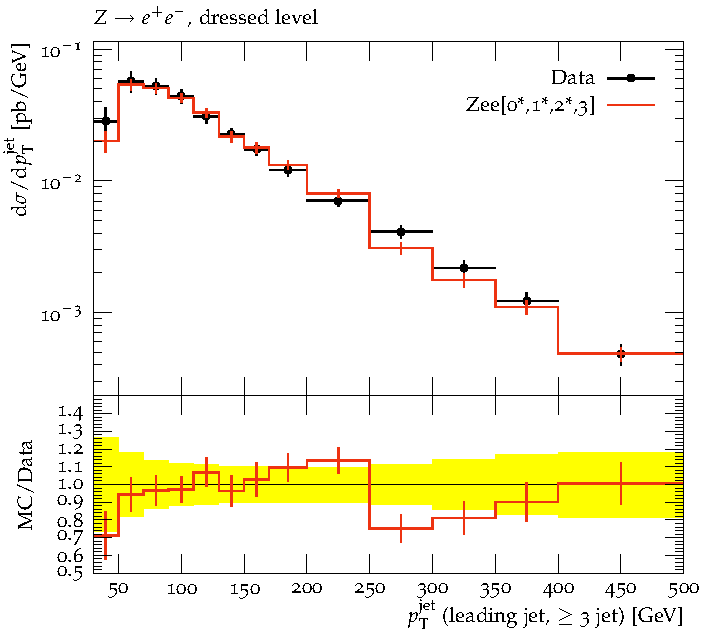
\includegraphics[width=0.85\linewidth]{Figures/ZMerging-13-3jpt.pdf}
    \caption{Transverse momentum of the third jet} 
    \label{fig7:d} 
  \end{subfigure} 
  \caption{Predictions of the production cross section of a Z+jets at s=$\sqrt{13}$ TeV using \code{Herwig 7.1.3}, in the electron decay channel. The predictions are compared to data (in black) corresponding to an integrated luminosity of 3.16 fb$^{-1}$ collected by ATLAS. The total measurement uncertainty is indicated by the yellow band, and the statistical uncertainties of the prediction are indicated by the error bars.}
  \label{fig7} 
\end{figure}

Figure \ref{fig9} gives the predictions for W + jets production at 7 TeV made in \code{Herwig 7.1.3}. The various different coloured samples correspond to different merging setups, as labelled in the legend, where the number indicates the additional merged legs and a * next to the number indicates NLO accuracy (LO otherwise). An aspect to note is that the mis-modelling of the red sample, which has the most additional parton emissions at LO and NLO accuracy, occurs seemingly sooner than the rest. Furthermore, while other samples undershoot, the red sample overshoots from $N_{\text{jets}}\geq3$ onwards. 

\begin{figure}[ht] 
  \begin{subfigure}[b]{0.5\linewidth}
    \centering
        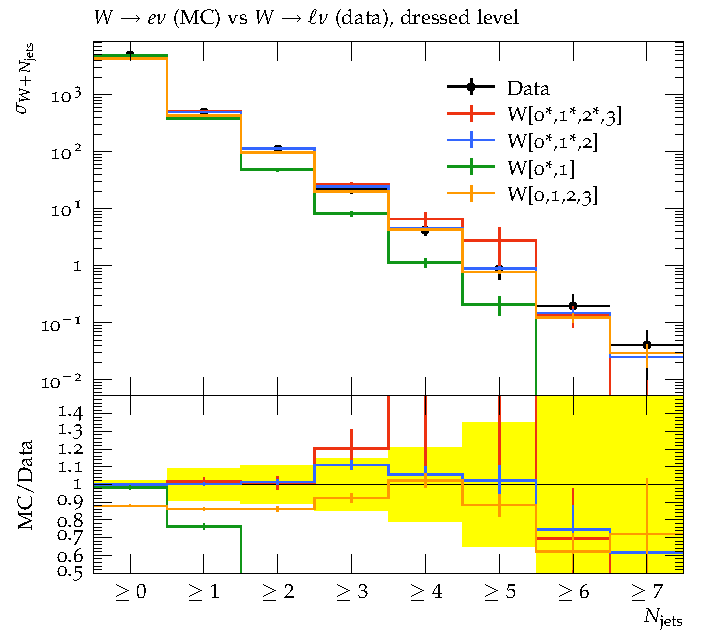
\includegraphics[width=0.85\linewidth]{Figures/WMerging-incl.pdf} 
    \caption{Inclusive jet multiplicity} 
    \label{fig9:a} 
    \vspace{4ex}
  \end{subfigure}%% 
  \begin{subfigure}[b]{0.5\linewidth}
    \centering
    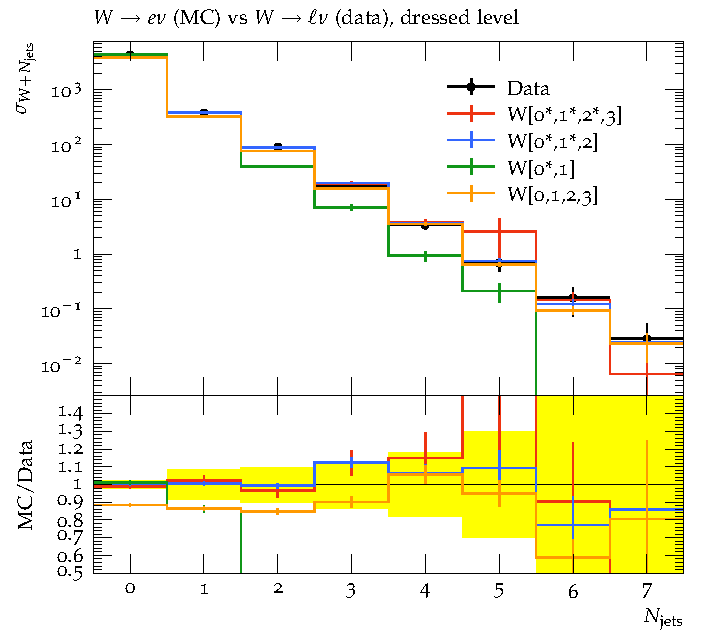
\includegraphics[width=0.85\linewidth]{Figures/WMerging-excl.pdf}
    \caption{Exclusive jet multiplicity} 
    \label{fig9:b} 
    \vspace{4ex}
  \end{subfigure} 
  \begin{subfigure}[b]{0.5\linewidth}
    \centering
    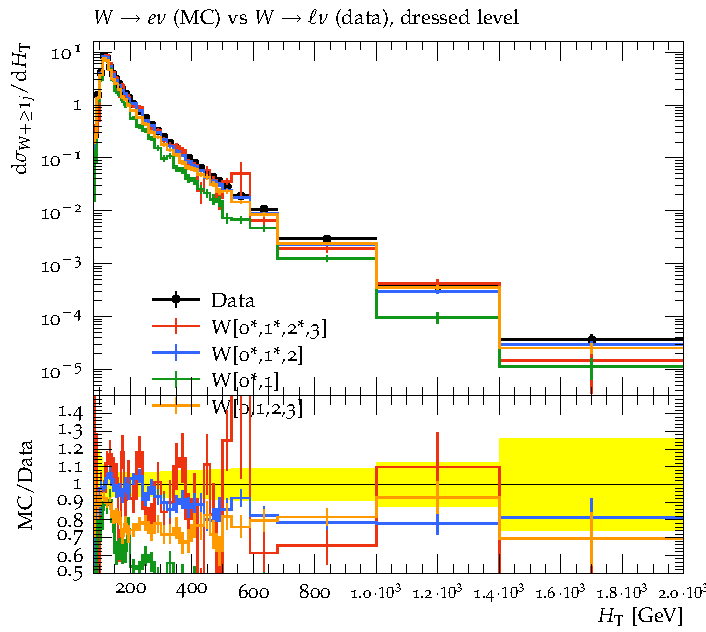
\includegraphics[width=0.85\linewidth]{Figures/WMerging-HT.pdf}
    \caption{Transverse hadronic activity} 
    \label{fig9:c} 
  \end{subfigure}%%
  \begin{subfigure}[b]{0.5\linewidth}
    \centering
    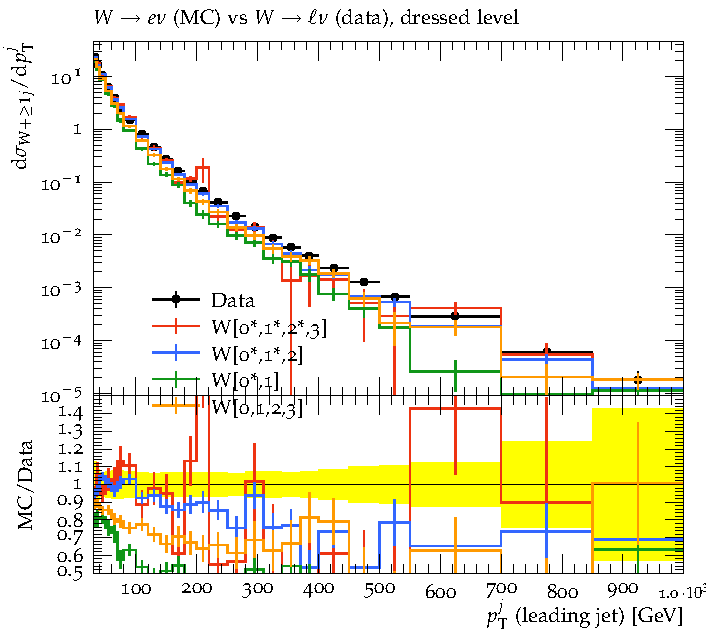
\includegraphics[width=0.85\linewidth]{Figures/WMerging-1jpt.pdf}
    \caption{Transverse momentum of the leading jet} 
    \label{fig9:d} 
  \end{subfigure} 
  \caption{Predictions of the production cross section of a W+jets at s=$\sqrt{7}$ TeV using \code{Herwig 7.1.3}, in the electron decay channel. The predictions are compared to data (in black) corresponding to an integrated luminosity of 4.6  fb$^{-1}$ collected by ATLAS. The total measurement uncertainty is indicated by the yellow band, and the statistical uncertainties of the prediction are indicated by the error bars.}
  \label{fig9} 
\end{figure}
